% Software Roboter (C++)
% Zuständig: Leander

\chapter{Software - Roboter}
\label{sec:software_robots}
\initials{LG}
Was die Ansteuerung der einzelnen Roboter angeht,
wird so so gut wie möglich dem DRY-Prinzip (``Don't repeat yourself'') gefolgt,
um Redundanzen zu vermeiden und dadurch den Wartungsaufwand möglichst gering zu halten.

\section{Kameras}
\label{subsec:robots_cams}
\initials{LG}
Es wird jeweils ein ESP32-CAM AI-Thinker Modul zur erweiterten
Fernüberwachung der Roboter verwendet.
%
Dieses verbindet sich über WLAN mit dem \texttt{IoT}-Netzwerk und bietet über HTTP einen MJPEG-Videostream an.
%
Die drei Videostreams (einer pro Roboter) werden dann im Web-Interface
zusätzlich zu den LiDAR-Umgebungsdaten angezeigt,
um das räumliche Vorstellungsvermögen der Benutzer zu unterstützen.
%
Die Videodaten werden also nicht automatisch verarbeitet und zur autonomen Steuerung verwendet,
sondern dienen nur als weiterer Input für die Bediener.
\begin{figure}[H]
    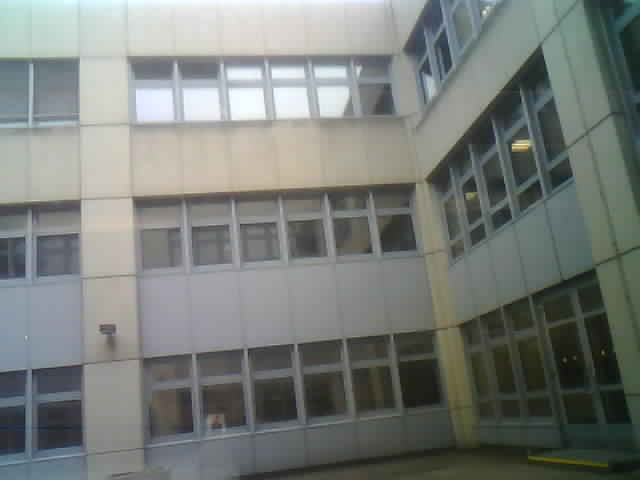
\includegraphics[width=0.7\textwidth, center]{img/cam_erstes_bild.png}
    \caption{Erstes empfangenes Bild der ESP32-CAM}
    \label{fig:cam_erstes_bild}
\end{figure}

\section{Core-Bibliothek}
\label{subec:robots_core}
\initials{LG}
Die Core-Bibliothek bildet eine weitere Abstrahierungsschicht zu den Funktionalitäten der Roboter-Hardware.
%
In diesem Modell stellt die Arduino-Bibliothek die erste Abstrahierungsschicht dar,
während die Core-Bibliothek diese weiter vereinfacht.
%
Durch diese Abstrahierung werden die Programme für die einzelnen Roboter um ein Vielfaches vereinfacht und dementsprechend übersichtlicher.
%
Die hier definierte Logik kann also für jeden Roboter wiederverwendet werden,
anstatt drei mal fast genau das Gleiche zu programmieren.
%
Die Core-Bibliothek übernimmt alles von der WLAN-Verbindung,
über die Fernsteuerung per WebSockets,
bis hin zum Umschalten der einzelnen Pins zur Ansteuerung der Motortreiber.
%
Die Programmierung der einzelnen Roboter beschränkt sich also darauf,
die einzelnen Komponenten zu konfigurieren und miteinander zu verbinden.
%
Da Herr Gastgeber während der Projektwoche 2023/24 (Siehe Abschnitt \ref{sec:vorgeschichte}) bereits viel Zeit darin investiert hat,
die Bibliothek so modular und wiederverwendbar wie möglich zu gestalten,
konnte diese mit nur wenigen Modifikationen für diese Diplomarbeit genutzt werden,
obwohl ein ganz anderer Hardwareaufbau verwendet wird.

\subsection{Module Allgemein}
\label{subsec:software_common_modules}
\initials{LG}
Wie schon erwähnt,
wurde die Core-Bibliothek so modular wie nur möglich gestaltet,
um so viele Anwendungsfälle wie möglich abzudecken.
%
Jedes Modul implementiert eine der folgenden Klassen:
\begin{itemize}
    \item \texttt{Sensor}: Ein Sensor bzw. eine Sensorgruppe
    \item \texttt{Actor}: Ein Aktor bzw. eine Aktorgruppe
    \item \texttt{Interface}: Ein Interface zur Steuerung, z.B. WLAN
\end{itemize}
Theoretisch ist es damit möglich,
gemeinsame Funktionalität für alle Sensoren/Aktoren/Interfaces zu definieren,
wobei dies aber nicht tatsächlich realisiert wurde.
%
Jede dieser Klassen implementiert wiederum die Klasse \texttt{Module},
welche die folgenden Funktionen definiert:
\begin{itemize}
    \item \lstinline[language=c]|void init()|:
        Ähnlich wie \texttt{setup()} beim Arduino, nur im Kontext eines einzelnen Moduls.
        Wird verwendet um das Modul zu initialisieren.
    \item \lstinline[language=c]|void tick()|:
        Ähnlich wie \texttt{loop()} beim Arduino, nur im Kontext eines einzelnen Moduls.
        Sobald der Roboter alle Module fertig initialisiert hat,
        wird ständig durch ebendiese Module iteriert,
        wobei deren \texttt{tick()}-Funktionen aufgerufen werden. 
    \item \lstinline[language=c]|void terminate()|:
        Wird eigentlich nicht verwendet,
        da die meisten Module nicht zur mehrfachen Initialisierung gedacht sind.
        Im Sinne der Vollständigkeit gibt es trotzdem die Möglichkeit,
        diese Funktion zu implementieren.
\end{itemize}
Außerdem stellt der Robota-Framework zwei Hilfsklassen (engl. ``Utilities''/``Utils'') zur Verfügung:
\texttt{KalmanFilter} und \texttt{PIDController}.

\subsection{Robota}
\initials{LG}
Die Klasse \texttt{Robota}%
\footnote{Dieser Name wurde in der Anfangsphase des Projekts (Ende 2023) gewählt, 
        um Konflikte mit der veralteten ``Arduino Robot Library'',
        welche standardmäßig von der Arduino IDE inkludiert wird,
        zu vermeiden.
        %
        Seit dem Wechsel von der Arduino IDE auf PlatformIO stellt dieser potentielle Konflikt kein Problem mehr da}
ist für das Management der Module zuständig.
%
Hierzu gibt es drei Variablen, welche für die Funktion zentral sind:
\begin{itemize}
    \item \lstinline[language=c]|uint32_t ticks|:
        Eine globaler Zähler, welche einmal pro Tick ausgeführt wird.
        Dieser kann von Modulen verwendet werden, um bestimmte Tätigkeiten nur alle $n$ Ticks auszuführen.
        % t is in microseconds: ((2^32) - 1) * (t * (10^-6)) / (60 * 60 * 24)
        Bei einer durchschnittlichen Zeit von ungefähr $t_{tick}=2700\mu s$ pro Tick reichen 32 Bits aus,
        um die Roboter für etwas mehr als $t_{overflow}=134$ Tage zu betreiben,
        was für die Zwecke dieses Projekts mehr als ausreichend sein sollte.
        \begin{equation*}
            t_{overflow} = (2^{32}-1) * t_{tick}
        \end{equation*}
    \item \lstinline[language=c]|uint16_t moduleTypes[MAX_MODULE_AMOUNT]|:
        Hier wird Typeninformation zu den Modulen gespeichert.
        %
        Diese wird in den Funktionen \texttt{getModule} und \texttt{getFirstModule} verwendet,
        um die Module nach Typ zu filtern.
    \item \lstinline[language=c]|Module *modules[MAX_MODULE_AMOUNT]|:
        Dies ist die gesamte Liste an registrierten Modulen.
        %
        Mit \texttt{addModule} können Einträge hinzugefügt werden.
\end{itemize}
%TODO: Robota funktionen; insb. init() und tick()

\subsection{Sensoren}
\subsubsection{LD20 LiDAR}
\initials{LG}
Der Code zum Auslesen des LiDAR-Sensors basiert auf zwei Informationsquellen zum Protokoll:
%
Die offizielle Dokumentation von youyeetoo \cite{youyeetoo-ld20},
und einer Arduino-Bibliothek namens LD14P\_RP2040 \cite{ld20-library},
welche sehr stark modifiziert wurde, um Teil des \textit{Robota}-Frameworks zu werden.

Die Daten des LiDARs werden über eine RS-232-Schnittstelle (230400 baud 8N1) ausgelesen.
%
Hierbei werden nur von Seiten des LiDARs Daten gesendet,
es gibt keine Möglichkeit diesen über die UART zu steuern.
%
Jede Nachricht beginnt mit einem Header-Byte \texttt{0x54},
gefolgt von einem Info-Byte,
welcher die Art des Pakets angibt.
\begin{table}[H]
    \centering
    \begin{tabular}{r|l}
    Info-Byte & Pakettyp   \\ \hline
    0x2C      & Sensordaten \\
    0xE0      & Systemstatus \\
    0x0F      & Herstellerinfos   
    \end{tabular}
    \caption{Pakettypen des LD20}
    \label{tab:ld20-packet-overview}
\end{table}
Jedes Paket ist von einem Prüfbyte zur Fehlererkennung mittels CRC%
\footnote{Cyclic Redundancy Check, ein Algorithmus zum Erzeugen von Prüfsummen}
gefolgt.
%
Nur Pakete mit Sensordaten werden tatsächlich verarbeitet,
alle anderen werden verworfen,
da sie für diesen Anwendungszweck nicht unbedingt nötig sind.
%
Ein Paket mit Sensordaten besteht (neben den oben beschriebenem Header, Info-Byte und CRC)
aus der Geschwindigkeit des Messkopfes,
dem Startwinkel der Messung,
12 Messpunkten,
dem Endwinkel der Messung,
und einem Zeitstempel.
%
Die Messpunkte bestehen nur aus der gemessenen Entfernung und Intensität;
der Winkel muss bei der Auswertung der Daten berechnet werden.
%
Bei allen Einträgen, die mehr als ein Byte beanspruchen,
wird das niederwertigste Byte zuerst übertragen.
%
Das Protokoll ist also little-endian,
was bedeutet, dass die Rohdaten direkt in den Arbeitsspeicher von z.B. einem Arduino oder ESP32 übernommen werden können.
\begin{table}[H]
    \centering
    \begin{tabular}{l|l|l}
    Name            & Typ           & Einheit  \\ \hline
    Header          & fixed 0x54    &   \\
    VerLen          & fixed 0x2C    &   \\
    Geschwindigkeit & UInt16        & deg/s \\
    Startwinkel     & UInt16        & 0.01°  \\
    Messdaten       & 12x Messdaten &    \\
    EndWinkel       & UInt16        & 0.01° \\
    Zeitstempel     & UInt16        & ms \\
    CRC             & 1 Byte        &
    \end{tabular}
    \caption{Paketformat des Messdatenpakets}
    \label{tab:ld20-measurement-packet}
\end{table}
\begin{table}[H]
    \centering
    \begin{tabular}{l|l|l}
    Name        & Typ       & Einheit   \\ \hline
    Distance    & UInt16    & mm        \\
    Intensity   & Uint8     &           \\ % Einheitslos
    \end{tabular}
    \caption{Format der rohen Messdaten}
    \label{tab:ld20-measurement-data}
\end{table}
Der Winkel $\alpha$ einer Messung kann mittels linearer Interpolation wie folgt berechnet werden:
\begin{equation}
    \alpha = \alpha_{s} + \frac{\alpha_{e}-\alpha_{s}}{n-1}*i = \alpha_{s} + \frac{\alpha_{e}-\alpha_{s}}{11}*i
\end{equation}
Hierbei repräsentieren $\alpha_{s}$ und $\alpha_{e}$ den Start- und Endwinkel der Messserie.
%
$n$ steht für die Anzahl der Messungen pro Messserie und ist bei dieser Anwendung konstant $12$,
weshalb $n-1$ auf $11$ vereinfacht werden kann.
%
$i$ ist der nullbasierte Index der jeweiligen Messung im Kontext der Messserie.

%\begin{tikzpicture}[node distance = 3cm]
%    \node [terminator, fill=blue!20] (start) {\textbf{Komplettes Packet empfangen}};
%    \node [process, below of=start] (crcCalc) {CRC berechnen};
%    \node [data, fill=blue!20, below of=crcCalc] (data) {Provide data};
%    \node [decision, fill=blue!20, below of=data] (crcCheck) {Daten gültig?};
%    \node [process, fill=red!20, right of=crcCheck, node distance=5cm] (error) {Paket verwerfen};
%    \node [process, fill=green!20, below of=crcCheck] (success) {Success};
%    \node [terminator, fill=blue!20, below of=success] (end) {\textbf{End}};
%    \path [connector] (start) -- (data);
%    \path [connector] (data) -- (crcCheck);
%    \path [connector] (crcCheck) -- node[anchor=south] {Nein} (error);
%    \path [connector] (crcCheck) -- node[anchor=east] {Ja} (success);
%    \path [connector] (error) |- (end);
%    \path [connector] (success) -- (end);
%\end{tikzpicture}


\subsubsection{Drehgeber}
\initials{LG}
Die beiden Drehgeber,
welche jeweils in den Motoren integriert sind,
werden von dem Modul \texttt{RotaryEncoder} ausgelesen.
%
Dieses Modul hat eine beim Kompilieren festgelegte Anzahl an sogenannten ``Ausgabe-Kanälen'',
da die Daten der Drehgeber an mehreren separaten Stellen verarbeitet werden müssen.
%
Die verwendete Zahl an Kanälen wurde auf Vier festgelegt, kann in der Zukunft aber sehr einfach geändert werden.
%
Anstatt die aktuelle Geschwindigkeit zu berechnen,
werden für jeden Kanal der Zeitpunkt des letzten Auslesens
und die Zahl an Impulsen vom Drehgeber seit ebendiesem Zeitpunkt gespeichert.
%
Dadurch können Module, welche die Daten verarbeiten,
selbst wählen, über welchen Zeitraum die Geschwindigkeit berechnet wird.
%
Das ist ein netter Nebeneffekt, aber eigentlich wurde dieser Ansatz gewählt,
weil das Datenformat zur Übertragung an den Server Daten in ebendiesem Format erwartet.
%
Da das Zählen selbst durch Interrupts gelöst wurde
und ISRs\footnote{Interrupt Service Routines}
nicht Mitglieder einer instanziierten Klasse sein dürfen (bzw. können),
muss zur Verwendung des \texttt{RotaryEncoder}-Moduls eine globale Funktion erstellt werden,
welche als ISR dient.
% TODO: function identifiers?
Diese Funktion soll einzig und allein \texttt{RotaryEncoder\#pulse()} aufrufen
und mittels \texttt{RotaryEncoder\#attachISR()} mit dem Trigger-Pin des Drehgebers ``verbunden'' werden.
%
\texttt{RotaryEncoder\#pulse()} regelt die Erhöhung der Zähler für alle Kanäle.
%
Beim Auslesen eines Kanals werden sowohl der Zeitstempel als auch der Zähler automatisch zurückgesetzt.

\subsubsection{MPU6050}
\initials{LG}
Da für das Auslesen der Rohdaten des eingebauten Gyroskops und Accelerometers
\texttt{MPU6050} eine externe Bibliothek \cite{adafruit-mpu6050} verwendet wurde,
war der Aufwand hierfür eher gering.
%
Das \texttt{MPU6050}-Modul sorgt also lediglich dafür,
dass die Werte nicht mehrmals pro Tick schnell hintereinander ausgelesen werden.
%
Erreicht wird das, indem ausgelesene Werte zwischengespeichert werden,
bis der aktuelle Tick vorbei ist.
%
Werden die Werte also mehrmals pro Tick abgefragt,
wird einfach der zuletzt ausgelesene Wert zurückgegeben.

\subsection{Aktoren}
\subsubsection{GenericDigitalOutput}
\initials{LG}
Das Modul \texttt{GenericDigitalOutput} dient als Grundlage zur Verwendung von anderen Modulen,
um einen digitalen Ausgang anzusteuern.

\subsubsection{PwmOutput}
\initials{LG}
Das Modul \texttt{PWMOutput} dient als Grundlage zur Verwendung von anderen Modulen,
um einen PWM-Ausgang anzusteuern.
%
Hierzu wird anstatt den standardmäßigen Arduino-Funktionen
direkt die ESP32 \texttt{ledc}-API verwendet,
um bestmögliche Konfigurationsoptionen zu erreichen \cite{esp32-ledc}. %TODO not sure if this sounds good
%
Es gibt es sowohl die Möglichkeit den Duty-Cycle direkt einzustellen,
oder anhand der erwünschten Breite des Impulses (in Mikrosekunden) zu berechnen;
dies ist insbesondere zum Einstellen vom Servomotoren nützlich.
%
Das Modul wählt automatisch den bestmöglichen PWM-Kanal:
%
Da sich beim ESP32 jeweils zwei PWM-Kanäle einen Timer teilen,
müssen diese die gleiche Frequenz haben.
%
Beim Initialisieren des PWM-Moduls wird automatisch nach einem Timer mit gleicher Frequenz gesucht,
welcher noch Platz für einen weiteren PWM-Kanal hat.
%
Wurde kein solcher Timer gefunden,
wird ein anderer konfiguriert.
%
Zu guter Letzt sorgt das PWM-Modul automatisch dafür,
dass die höchstmögliche Auflösung verwendet wird.
%
Die PWM-Kanäle des ESP32 haben eine zur Frequenz indirekt proportionale Auflösung \cite{esp32-technical-reference}.
Die maximale Signalfrequenz $f_{out}$ bei gegebener Auflösung $R$ lässt sich wie folgt berechnen:
\begin{equation}
    f_{out} = \frac{f_{clk}}{N*2^{R}}
\end{equation}
Daraus ergibt sich zur Berechnung der maximalen Auflösung bei gegebener Signalfrequenz:
\begin{equation}
    R = \log_2\left( \frac{f_{clk}}{f_{out}*N} \right)
\end{equation}
Hierbei ist $f_{clk}$ das gegebene Taktsignal des Timers und $N$ der Wert des Prescalers.
%
$R_{max}$ wird abgerundet.

Zur Berechnung der höchstmöglichen Auflösung $R_{max}$ wird $N=1$ gesetzt und das Ergebnis abgerundet.
%
Zu beachten ist hierbei,
dass alle Ergebnisse auf einen Maximalwert von 20 limitiert sind.
% ^ TODO komische docs
%
Tatsächlich gibt es auch eine minimale Auflösung,
wobei es ja immer möglich ist,
die Auflösung eines Signals künstlich zu verringern.
%
Die minimale Auflösung kann berechnet werden, indem $N=1023+\frac{255}{256}$ gesetzt wird.
Das Ergebnis wird aufgerundet und hat einen Minimalwert von 1.

Bei Verwendung der \texttt{APB\_CLK}, mit 80MHz als Taktsignal,
ergeben sich also folgende Werte:
\begin{table}[H]
    \centering
    \begin{tabular}{r|l|l}
    $f_{sig}$ [Hz]  & $R_{max}$ [bits] & $R_{min}$ [bits] \\ \hline
    1k        & 16 & 7 \\
    2k        & 15 & 6 \\
    5k        & 13 & 4 \\
    10k       & 12 & 3 \\
    20k       & 11 & 2 \\
    50k       & 10 & 1 \\
    100k      & 9  & 1 \\
    1M        & 6  & 1 \\
    2M        & 5  & 1 \\
    5M        & 4  & 1 \\
    \end{tabular}
    \caption{PWM-Auflösungen bei gewählten Frequenzen}
    \label{tab:pwm-resolution}
\end{table}

\subsubsection{SingleMotorOutput}
\initials{LG}
Das Modul \texttt{SingleMotorOutput} verwendet die bereits beschriebenen Module
\texttt{GenericDigitalOutput} und \texttt{PWMOutput},
um einen einzelnen Motor mittels eines Motortreibers anzusteuern.
Um die Verwendung mit möglichst vielen unterschiedlichen Motortreibern zu gewährleisten,
gibt es drei unterschiedliche Möglichkeiten, die \texttt{GenericDigitalOutput}s zu konfigurieren:
\begin{itemize}
    \item Verwendung eines Pins für \texttt{forward}
    \item Verwendung eines Pins für \texttt{backward}
    \item Verwendung beider Pins
\end{itemize}
In Kombination mit dem Tumbller wurde die erste der drei Möglichkeiten gewählt.
%
Der eingebaute Motortreiber erwartet zwar sowohl ein \texttt{forward}- als auch ein \texttt{backward}-Signal,
jedoch wird das \texttt{backward}-Signal hardwaremäßig durch Inversion von \texttt{forward} generiert.
%
Die Richtung und Geschwindigkeit werden als signierte 16-Bit Integer gegeben,
wobei negative Werte als Rückwärtsfahren interpretiert werden.
%
Es bleiben also 15 Bits Genauigkeit für die Geschwindigkeit,
was mehr als ausreichend ist.
%
Das \texttt{SingleMotorOutput}-Modul stellt lediglich eine Steuerung dar,
die Regelung der Motorgeschwindigkeit mit Rückkopplung durch Drehgeber wird andernorts realisiert.

\subsubsection{BalanceController}
\initials{LG}
Die Gesamtheit der Aktoren kommt im \texttt{BalanceController} zusammen:
Hier werden die Daten vom \texttt{MPU6050} ausgelesen,
zur Glättung durch einen Kalman-Filter (siehe Abschnitt \ref{subsubsec:kalman}) gefiltert,
und als Rückkopplung in einen PID-Regler eingegeben,
welcher mittels zwei \texttt{SingleMotorOutput}s die beiden Motoren kontrolliert.
%
Als Führungsgröße wird hier zusätzlich die gewollte Geschwindigkeit und Auslenkung eingegeben,
welche vom Server an die Roboter gesendet wird.

TODO mehr Beschreibung 

\subsection{Interfaces}
\subsubsection{WiFiConnection}
\initials{LG}
Dieses Modul ist zuständig für die Steuerung der WLAN-Verbindung.
%
Die Zugangsdaten des Netzwerks können während dem Kompilieren
als Umgebungsvariablen zur Verfügung gestellt werden.
%
In der HTL Ettenreichgasse wird das \texttt{IoT}-Netzwerk verwendet.
% TODO 13:50
Im Konstruktor des Moduls wird es mit dem erwünschtem Hostnamen des Geräts
und den Details zur Verbindung mit dem WLAN-Netzwerk (SSID/Passwort) versorgt.
%
Bei Initialisierung des Moduls wird die private Funktion \texttt{attemptConnection()} aufgerufen,
welche alle Schritte zur Verbindung mit dem gegebenem Netzwerk erledigt.
%
Hierbei wird zu Debugging-Zwecken eine Liste aller verfügbaren Netzwerke über die UART ausgegeben.
%
Bei erfolgreicher Verbindung mit einem Netzwerk wird außerdem die eigene IP-Adresse über die UART ausgegeben. 

\subsubsection{WebSocketControls}
\initials{LG}
Die WebSocketControls dienen als Wrapper zur \texttt{ESPAsyncWebServer}-Bibliothek,
mit welcher auf Port 80 ein asynchroner Webserver zur Verfügung gestellt wird,
der unter dem Pfad \texttt{/ws} WebSocket-Verbindungen (siehe Kapitel \ref{sec:websockets}) akzeptiert.
%
Sobald sich ein Client mit dem WS-Server verbindet,
können mittels Callback-Funktionen Befehle empfangen werden.
%
Mittels der Funktion \texttt{WebSocketControls::send(Wrapper *message)} können Daten an den Client gesendet werden.
%
Ein Client wäre in diesem Anwendungsfall der zentrale Server,
welcher die Roboter kontrolliert.
%
Hier ist die Terminologie leider etwas verwirrend.
%
Theoretisch wäre es möglich,
die Roboter als Clients agieren zu lassen,
was aber den nachteil hätte,
das die URL des Servers zum Zeitpunkt des Kompilieren bekannt sein müsste.
%
Stattdessen muss der Server (welcher als WS-Client agiert) nur die aktuelle IP-Adressen der Clients wissen,
welche man leicht bzw. schnell in der Konfiguration des Servers ändern kann.

\subsection{KalmanFilter}
\label{subsubsec:kalman}
\initials{LG}
Kalman-Filter werden allgemein zu Schätzung von Systemzuständen verwendet,
welche nur ungenau gemessen werden können.
%
Die konkrete Anwendung in diesem Projekt beschränkt sich auf die Berechnung
der Neigung der Roboter basierend auf den relativ ungenauen Messdaten des MPU6050.
%
Hierbei werden die Daten des Gyroskops mit denen des Accelerometers kombiniert,
um eine möglichst genaue Schätzung des Neigungswinkel zu erreichen\cite{digikey-kalman}.
%
Diese sogenannte Sensorfusion ermöglicht es,
die Messfehler der beiden Sensoren auszugleichen,
um einen genauen Wert zu erreichen.
%
Der verwendete Code zum Kalman-Filter basiert auf einem modifiziertem Beispielcode von Kristian Lauszus \cite{lauszus}.
% TODO maths?

\subsection{PIDController}
\initials{LG}
PID-Regler (Proportional, Integral, Differential) werden verwendet,
um eine Regelstrecke bestmöglich zu regeln.
%
Im Kontext der Tumbller werden PID-Regler an zwei Stellen eingesetzt:
\begin{itemize}
    \item Regelung der Motorgeschwindigkeit
    \item Regelung der Neigung und Auslenkung der Roboter
\end{itemize}

\subsubsection{Theorie}
\initials{LG}
Im Model des Standardregelkreises ist der PID-Regler,
wie der Name schon impliziert,
an der Position des Reglers einzusetzen.
%
Der Standardregelkreis besteht aus
der Führungsgröße (dem Sollwert) $w(t)$,
der Regelgröße (dem Istwert) $x(t)$,
der Regelabweichung $e(t)=w(t)-x(t)$,
und der Stellgröße $u(t)$.
%
Regler akzeptieren im Allgemeinen die Regelabweichung $e(t)$ als Eingang und
geben die Stellgröße $u(t)$ aus.
%
Die Aufgabe des Reglers besteht normalerweise darin,
die Regelabweichung so gut wie möglich zu minimieren.
\begin{figure}[H]
    \centering
    \begin{tikzpicture}[auto, node distance=2.5cm, >=Latex]
      % define style of blocks
      \tikzstyle{block} = [
        draw, rectangle, minimum height=1cm,
        minimum width=2cm, align=center]

      % Eingang (Führungsgröße)
      \node[] (w) {};
      % Summierer
      \node[circle, draw, minimum size=0.6cm, right=2cm of w] (sum) {};
      % Regler
      \node[block, right=2cm of sum] (regler) {Regler};
      % Regelstrecke
      \node[block, right=2cm of regler] (strecke) {Regelstrecke};
      % x verbindung
      \node[coordinate, right=2cm of strecke] (x_knot) {};
      % x Ausgang
      \node[coordinate, right=0.8cm of x_knot] (x_output) {};
      % helper node
      \node[coordinate, below=2cm of sum] (x_corner) {};

      \draw[->] (w) -- node[above] {\(w(t)\)} (sum);
      \draw[->] (sum) -- node[above] {\(e(t)\)} (regler);
      \draw[->] (regler) -- node[above] {\(u(t)\)} (strecke);
      \draw[-] (strecke) -- node[above] {\(x(t)\)} (x_knot);
      \fill (x_knot) circle[radius=1mm];
      \draw[->] (x_knot) -- (x_output);
      \draw[-] (x_knot) |- node[above,pos=0.75] {Rückführung}
                           node[below,pos=0.75] {\(x(t)\)} (x_corner);
      \draw[->] (x_corner) -| node[pos=0.98, right] {$-$} (sum);
    \end{tikzpicture}
    \caption{Standardregelkreis}
    \label{fig:allgemeiner-regelkreis}
\end{figure}
Digitale (bzw. diskrete) PID-Regler lassen sich sehr einfach implementieren:

% P
\begin{equation}
    u_P[k] = e[k]
\end{equation}
% I
\begin{equation}
    u_I[k] = u_I[k-1] + e[k] * \Delta t
\end{equation}
% D
\begin{equation}
    u_D[k] = \frac{e[k] - e[k-1]}{\Delta t}
\end{equation}
% combined
\begin{equation}
    u[k] = k_P * u_P[k] + k_I * u_I[k] + k_D * u_D[k]
\end{equation}

Hierbei ist $e[k]$ die aktuelle Regelabweichung,
während $u[k]$ die Stellgröße repräsentiert.
%
$k_P$, $k_I$, und $k_D$ sind Verstärkungsfaktoren,
mit denen man den Regler einstellen kann,
indem der Einfluss der jeweiligen Anteile
auf das Ausgangssignal $u[k]$ variiert wird.
%
Diese drei Konstanten richtig zu wählen,
ist notwendig,
damit der Regler optimal funktioniert. 
%
Die Größe $\Delta t$ bezeichnet die Abtastzeit und wird zur zeitdiskreten
Berechnung des Integral- und Differentialanteils benötigt.

\subsubsection{Praxis}
In C-Code implementiert schaut das dann wie folgt aus:
\begin{lstlisting}[caption={Implementierung des PID-Reglers in C},label=lst:pid]
float PIDController::pid(float error, float dt) {
  static float integral, previous;

  // P
  float proportional = error;
  // I
  integral += error * dt;
  // D
  float derivative = (error - previous) / dt;
  previous = error;

  return (kp * proportional) +
         (ki * integral) +
         (kd * derivative);
}
\end{lstlisting}
Listing \ref{lst:pid} ist ein Ausschnitt aus der \texttt{PIDController} Klasse,
in welcher die drei schon vorhin erwähnten Verstärkungsfaktoren als globale Variablen definiert sind.
%  
Es ist zu beachten,
dass \texttt{error}
jede gewünschte Einheit haben kann,
solange der Code,
der \texttt{PIDController::pid} aufruft,
den zurückgegebenen Wert korrekt verarbeitet.
%
Der Standardisierung halber wird empfohlen,
dass \texttt{dt} (delta time) in Sekunden angegeben wird,
allerdings ist es theoretisch möglich,
jegliche Zeiteinheit zu verwenden. 
%
Der Code zum PID-Regler wurde absichtlich so abstrakt wie möglich gehalten,
um die Möglichkeit zur Verwendung in vielen unterschiedlichen Situationen zu gewährleisten.

\section{Guide}
\label{subsec:software_guide}
\initials{LG}
Die Software von Guide ist in diesem Projekt in dem Sinne einzigartig,
dass,
zusätzlich zur Steuerung des Roboters selber,
die gemessen LiDAR-Werte empfangen,
aufbereitet,
und mit möglichst wenig Verzögerung an den Server weitergeleitet werden müssen.
%
Der Erfolg des ganzen Projekts ist also von der Verlässlichkeit dieser Software abhängig.
%
Abgesehen davon verhält sich der Guide eigentlich genau gleich wie Tamerlan und Bambi:
%
Befehle werden vom Server empfangen und ausgeführt,
Messwerte werden an den Server weitergeleitet.
%
Da auch die Aufbereitung der LiDAR-Daten bereits in der Core-Bibliothek realisiert wurde,
ist die Software für den Guide ebenso wie bei den anderen Robotern sehr schnell zusammengestellt.

\section{Tamerlan \& Bambi}
\label{subsec:software_tamerlan}
\initials{LG}
Da Tamerlan und Bambi über identische Hardware verfügen,
ist auch deren Code fast gleich:
%
Der einzige Unterschied besteht im Hostnamen, welcher für die WLAN-Verbindung gesetzt wird:
%
Bei Tamerlan lautet dieser \texttt{sb-tame}, bei Bambi \texttt{sb-bambi}.